\documentclass[12pt,a4paper]{article}
\usepackage[latin1]{inputenc}
\usepackage{amsmath}
\usepackage{amsfonts}
\usepackage{uarial}
\usepackage{amssymb}
\usepackage{graphicx}
\author{Miguel Hernández Boza}
\title{GRecommender}
\begin{document}
	
		\maketitle
		\begin{abstract}
			
			En la siguiente memoria voy a explicar cómo he desarrollado mi sistema de recomendaciones de películas, qué datos he utilizado y cómo he ido eligiendo todas las partes de mi solución.\\
			
			El nombre que le he dado a mi solución es GRecommender. Éste se basa en un sistema de recomendaciones con una base de datos orientada a grafos que da soporte a todo el sistema. El frontal interactúa con la base de datos modificando ésta creando nuevos vértices al insertar un nuevo usuario y aristas en el caso de las recomendaciones. \\
			
			En las siguientes páginas se describirá todo el proceso que se ha seguido hasta lograr la solución.\\
			
		\end{abstract}
		\clearpage
		\tableofcontents
		\clearpage
		\listoffigures
		\clearpage
		\section{Metodología de trabajo}
		
			La metodología usada para esta solución es la CRISPDM.
			\begin{itemize}
			\item \textit{Comprensión del negocio}: 			
			Esta fase inicial se centra en la comprensión de los objetivos y requisitos del proyecto. En este caso, el de una solución que de recomendaciones de películas. Para lograr esto recibiremos como fuente dé información a Filmaffinity a través de un scraper implementado en Java. El valor que puede tener esta solución sería la de ganar más relevancia con nuestras recomendaciones, ya que podemos ser una página de referencia a la hora de hablar sobre cine a través de unas recomendaciones dinámicas y teniendo en cuenta las acciones de los usuarios.
			\item \textit{Comprensión de Datos}: 
			Esta fase comienza con una colección inicial de datos y procesos con actividades con el objetivo de familiarizarse con los datos. Dentro de esta información tendremos la sinopsis de la película, actores que aparecen, director de la película o sinopsis y nota que se le da a la película. Por otro lado, nos aparecerán también comentarios positivos o negativos que nos harán ver una sensación global sobre cada película. Además de esto tendremos diferentes etiquetas sobre cada película que nos pueden servir para buscar películas similares.
			\item \textit{Preparación de datos}: 
			La preparación de los datos ha sido a partir de un scraper en Java. El funcionamiento es el siguiente: busqué información sobre Filmaffinity y encontré un articulo donde se realizó un análisis sobre las notas recibidas, en este articulo aparecía un código en Perl donde descargaba las páginas de la web. He seleccionado los id de las películas para realizar de nuevo las peticiones pero esta vez he descargado toda la siguiente información por película de Filmaffinity.\\
			
			\subitem - Título original
			\subitem - Año
			\subitem - Duración
			\subitem - País
			\subitem - Guión
			\subitem - Música
			\subitem - Fotografía
			\subitem - Genero
			\subitem - Productora
			\subitem - Reparto
			\subitem - Director
			\subitem - Simbiosis
			\subitem - Calificación
			\subitem - Comentarios
			
			También me he descargado una base de datos de comentarios para ver si algunas de ellas coincidían con las películas que ya tenía para tener mayor cantidad de datos posibles.
			Además, con estos comentarios, podría conseguir calificaciones positivas o negativas, extrayendo esta información de los textos a través de NLP (Natural Language Processing) y la rama del análisis del sentimiento.
			\item \textit{Modelado}: 
			Para modelar los datos, al ir a utilizar como base de datos una no relacional, orientada a grafos. He preparado distintos CSV desde los cuales importaré toda la información estática. Tendré un esquema desde el que comenzaré a insertar los usuarios que recibirán las primeras recomendaciones basadas en los mayores calificaciones.
			
			Este modelo vendrá descrito en el diseño de la base de datos.
			\item \textit{Evaluación}: 
			El modelo seguido para la solución es la siguiente. Inicialmente tenemos toda la información de películas insertada en la base de datos, esta tendrá el siguiente esquema.
			
			Una vez queramos registrarnos en la aplicación, ésta creara una entidad o nodo con los datos del usuario y basará las primeras recomendaciones en los valores más altos de evaluación de cada género de película. Esto lo lograremos creando relaciones de esta entidad con los nodos de esas películas. 
			
			Una vez el usuario entre, verá esas recomendaciones y podrá decidir cuáles le interesa, con ello editaremos esas relaciones borrando las que no le interesen y enseñándole otras con similitudes en diferentes parámetros como los que hemos visto anteriormente, por ejemplo:

			\subitem - Año
			\subitem - Genero
			\subitem - Actores que aparecen
			\subitem - Director
			
			Si elige nuevas películas en las que está interesado se crearán estas nuevas relaciones y se le podrán mostrar más. Siempre se podrá volver a empezar o buscar libremente las películas para después comenzar el método de recomendación.
			\item \textit{Despliegue}: 
			Para el despliegue será necesario un servidor Apache Tomcat para la parte del frontend con una base de datos Neo4j como backend junto con una API que conecte el frontend con el backend. 
			Para mandar las órdenes desde el backend utilizaremos curl para generar la petición POST que es necesaria para crear/editar/borrar partes de la base de datos.		
			
		\end{itemize}
		\clearpage
		\section{Fuentes de datos}
		
		La fuente de datos viene a partir de dos lugares, hemos utilizado un scraper en Java para descargar toda la información de cada película de Filmaffinity y por otro lado hemos utilizado los datos de un proyecto open-source donde se realizaban diferentes opiniones para ver si podíamos añadir más información a las películas.\\
		
		El scraper realiza lo siguiente:
		
		\begin{verbatim}
		
		// Descarga de peliculas a a través del identificador.
		archivo = new File ("C:\\Users\\Miguel\\GRecommend\\indices_min.txt");
		fr = new FileReader (archivo);
		br = new BufferedReader(fr);
		// Fichero de salida
		fichero = new FileWriter("C:\\Users\\Miguel\\GRecommend\\Pelis.csv");
		pw = new PrintWriter(fichero);
		
		// Lectura del fichero
		String id;
		while((id=br.readLine())!=null){
		
		try {
		doc = Jsoup.connect("http://www.filmaffinity.com/es/film"+id+".html").get();	
		
		// Formato csv:
		// Titulo,año, duracion,país,Director,Guión,Música,Fotografía,Reparto
		Element content = doc.getElementById("left-column");
		Element rate = doc.getElementById("movie-rat-avg");
		String linea_wr = content.text();
		linea_wr = linea_wr.replaceAll("Título original ", "");
		linea_wr = linea_wr.replaceAll(" Año ", ";");
		...
		
		\end{verbatim}
		\begin{itemize}
		\item Tenemos un primer fichero con id's válidos de películas de filmaffinity, como se ha comentado anteriormente.
		\item Estos id's se concatenan con la URL a la que vamos a realizar la petición y lo parseamos con la librería jsoup
		\item Tratamos lo que nos devuelve extrayendo los parámetros que nos interesan y generando el CSV.		
		\end{itemize}
		
		En total tenía más de 40.000 índices de películas pero para esta solución he reducido simplemente a 100 identificadores, el resultado es el mismo salvo por los tiempos de procesado e importación, pero el modelo no cambia.
		
		La salida en CSV nos queda de la siguiente manera:
		\begin{verbatim}
		
		Nachtgestalten (Nightshapes);1999;104 min.;Alemania;
		Andreas Dresen;Andreas Dresen;Cathrin Pfeifer, Rainer Rohloff;
		Andreas Höfer;Meriam Abbas, Dominique Horwitz, Oliver Bäbler, 
		Susanne Bormann, Michael Gwisdek, Ricardo Valentim;
		European Script Fund / Film Board Berlin Brandenburg
		 / Studio Babelsberg Independents;
		Drama;Retrata la vida de un grupo de desheredados de Berlín.
		\end{verbatim}
		
		De este generamos otro para crear las relaciones entre géneros de las películas y estas.
	
		Una vez tenemos este CSV, preparamos los diferentes CSV para importar en Neo4j. Para ello creamos un fichero de carga que lo vaya leyendo y realizado las peticiones curl necesarias para importar cada entidad en forma de nodo, y las relaciones que existen.
		Esto lo veremos en la sección de base de datos.
		\clearpage
		Una vez realizado esto, tenemos el siguiente grafo sobre el que trabajar. Todo esta última parte viene explicado en detalle en el diseño de la base de datos.

		\begin{figure}[tbph!]
			\centering
			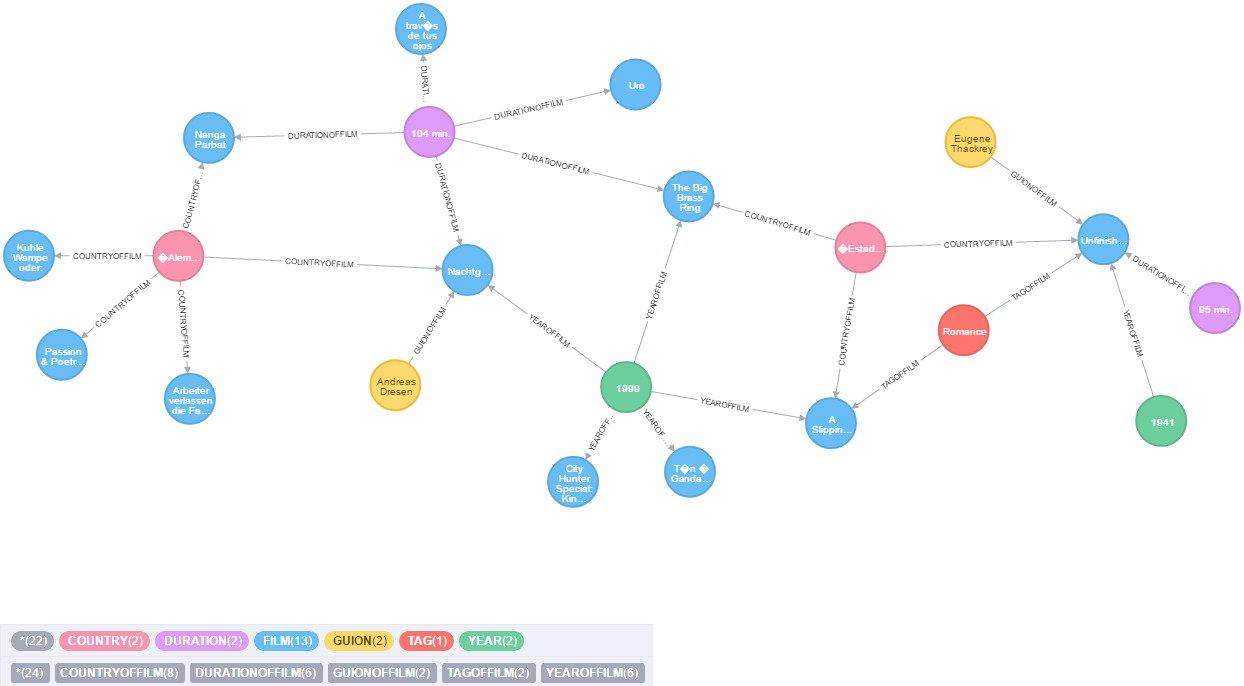
\includegraphics[width=1\linewidth]{images/Grafo_Peliculas.png}
			\caption{Grafo inicial.}
			\label{fig:GrafoInicial}
		\end{figure}
		
		A este será al que le añadamos los usuarios y crearemos sus relaciones como forma de crear estas recomendaciones.
		\clearpage
		\section{Diseño de arquitectura SW}
		
		La arquitectura estará basada en sistemas distribuidos, donde tendremos una arquitectura cliente-servidor. En el servidor recibiremos las peticiones de usuarios para conectarse y en el cliente podremos realizar las modificaciones en las recomendaciones que se nos entreguen.\\
		
		El servidor tendrá instalado la instancia de Neo4j donde almacenaremos los datos, y un Tomcat para el frontal web. Los usuarios realizarán la conexión a este frontal y será necesario un login para acceder. 
		Este frontal estará basado en D3 para la visualización junto a AngularJS.\\
		
		En la siguiente imagen se explica como sería el la arquitectura.
		
		\begin{figure}[tbph!]
			\centering
			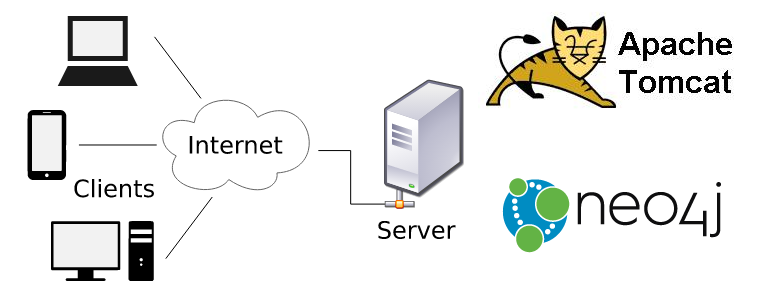
\includegraphics[width=1\linewidth]{images/Arq_clientserver.png}
			\caption{Arquitectura Cliente Servidor.}
			\label{fig:Arq-client-serv}
		\end{figure}
		\clearpage
		Para la comunicación entre el Tomcat y Neo4j usaremos la biblioteca Neo4j - OGM de Java que puede persistir en objetos de dominio utilizando Neo4j. Utiliza declaraciones Cypher para manejar esas operaciones en Neo4j.
		
		El MDS es compatible con el control de cambios para reducir al mínimo las actualizaciones necesarias y persistencia transitiva (lectura y actualización de los barrios de un objeto).
		
		La conexión con Neo4j manejado por una capa de conductor, que puede utilizar el protocolo binario , HTTP o API integradas de Neo4j.\\
		La siguiente figura explica como seria toda la arquitectura de GRecommender.\\
		
		
		\begin{figure}[tbph!]
			\centering
			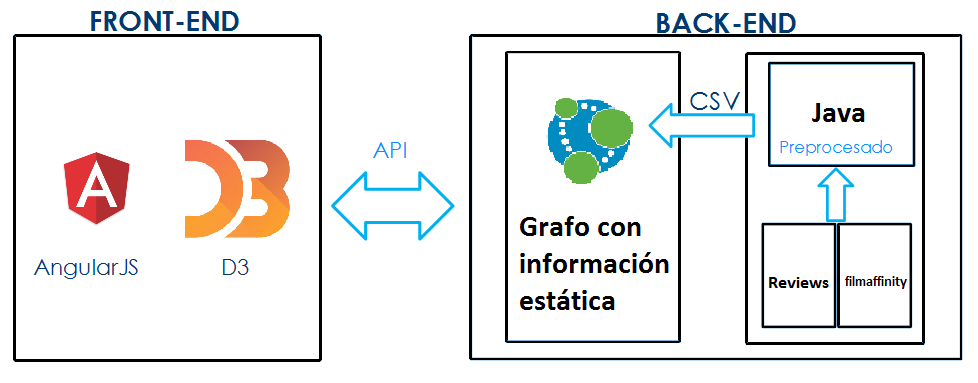
\includegraphics[width=1\linewidth]{images/Arquitect_GRecommend.png}
			\caption{Esquema CRISP-DM.}
			\label{fig:EsquemaCRISPDM}
		\end{figure}
		\clearpage
		\section{Diseño de la base datos}
		
		En esta solución hemos implementado como base de datos una orientada a grafos, para poder aprovechar la teoría de grafos a la hora de realizar las recomendaciones.\\
		
		La eficacia de los grafos se basa en su gran potencia de abstracción y la muy clara representación de cualquier relación (de orden, precedencia, etc) lo que facilita enormemente tanto la fase de modelado como de resolución del problema. Gracias a la Teoría de Grafos se han desarrollado una gran variedad de algoritmos eficientes que nos permiten tomar una mejor decisión.\\	
		
		Una base de datos orientada a grafos (BDOG) representa la información como nodos de un grafo y sus relaciones con las aristas del mismo, de manera que se pueda usar teoría de grafos para recorrer la base de datos ya que esta puede describir atributos de los nodos (entidades) y las aristas (relaciones).\\
		
		Con estas nuevas bases de datos, la información se almacena de un modo diferente, se pueden combinar distintas fuentes de información de un modo sencillo, reduciendo el tamaño de la base de datos y optimizando las consultas que de otro modo serían muy costosas.
		
		Neo4j es una base de datos orientada a grafos nativa altamente escalable que aprovecha las relaciones de datos como entidades de primera clase, para ayudar a las empresas a crear aplicaciones inteligentes para satisfacer los desafíos de datos actuales en constante evolución.\\
		
		\begin{figure}[tbph!]
			\centering
			
\includegraphics[width=0.5\linewidth]{images/neo4j_notag_whitebg}
			\caption{Neo4j.}
			\label{fig:Neo4j}
		\end{figure}
		\clearpage
		
		Para importar los datos utilizaremos el método que nos proporciona la propia base de datos Neo4j. Mediante el comando nativo LOAD CSV podemos cargar un CSV externo y crear nuestros nodos y relaciones que deseemos por cada elemento de la fila.\\
		
		El lenguaje que utiliza Neo4j para las consultas e importación de los datos es Cypher.
		Cypher es un lenguaje declarativo, inspirado en SQL para describir los patrones en los grafos visualmente utilizando una sintaxis ASCII-art.\\
		
		Esto nos permite afirmar lo que queremos seleccionar, insertar, actualizar o eliminar de nuestros datos del gráfico sin necesidad de nosotros para describir exactamente cómo hacerlo.
		
		\begin{figure}[tbph!]
			\centering
			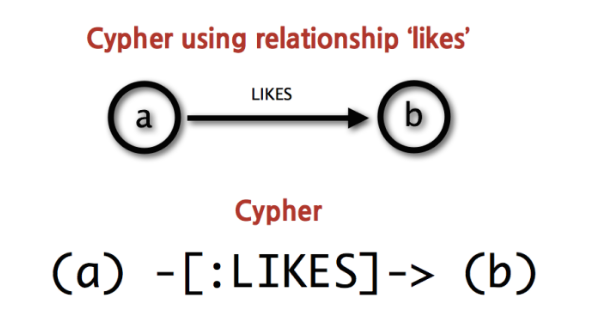
\includegraphics[width=0.5\linewidth]{images/cypher}
			\caption{Cypher.}
			\label{fig:Cypher}
		\end{figure}
		
		Los comandos en cypher serían los siguientes:
		
		\begin{verbatim}
		LOAD CSV FROM 'file:///Pelis.csv' AS line FIELDTERMINATOR ';' 
		CREATE (f:FILM {name:line[1], score:line[0]})
		
		LOAD CSV FROM 'file:///Pelis.csv' AS line FIELDTERMINATOR ';' 
		MERGE (y:YEAR {date:toInt(line[2])})
		
		LOAD CSV FROM 'file:///Pelis.csv' AS line FIELDTERMINATOR ';' 
		MERGE (d:DURATION {min:line[3]})
		
		LOAD CSV FROM 'file:///Pelis.csv' AS line FIELDTERMINATOR ';' 
		MERGE (c:COUNTRY {name:line[4]})
		
		LOAD CSV FROM 'file:///Pelis.csv' AS line FIELDTERMINATOR ';' 
		MERGE (dir:DIRECTOR {name:line[5]})
		
		LOAD CSV FROM 'file:///Pelis.csv' AS line FIELDTERMINATOR ';' 
		MERGE (g:GUION {name:line[6]})
		
		LOAD CSV FROM 'file:///Pelis_TAGS.csv' AS line FIELDTERMINATOR ';' 
		MATCH (f:FILM {name:line[0]})
		MERGE (t:TAG {tag:line[1]})
		MERGE (f)<-[:TAGOFFILM]-(t)
		
		LOAD CSV FROM 'file:///Pelis.csv' AS line  FIELDTERMINATOR ';' 
		MATCH (f:YEAR {date:toInt(line[2])}), (film:FILM {name:line[1]})
		CREATE (f)-[:YEAROFFILM]->(film)
		
		LOAD CSV FROM 'file:///Pelis.csv' AS line  FIELDTERMINATOR ';' 
		MATCH (d:DURATION {min:line[3]}), (film:FILM {name:line[1]})
		CREATE (d)-[:DURATIONOFFILM]->(film)
		
		LOAD CSV FROM 'file:///Pelis.csv' AS line  FIELDTERMINATOR ';' 
		MATCH (c:COUNTRY {name:line[4]}), (film:FILM {name:line[1]})
		CREATE (c)-[:COUNTRYOFFILM]->(film)
		
		LOAD CSV FROM 'file:///Pelis.csv' AS line  FIELDTERMINATOR ';' 
		MATCH (dir:DIRECTOR {name:line[5]}), (film:FILM {name:line[1]})
		CREATE (dir)-[:DIRECTOROFFILM]->(film)
		
		LOAD CSV FROM 'file:///Pelis.csv' AS line  FIELDTERMINATOR ';' 
		MATCH (g:GUION {name:line[6]}), (film:FILM {name:line[1]})
		CREATE (g)-[:GUIONOFFILM]->(film)
		\end{verbatim}
		
		
		Un ejemplo de una petición curl:
		
		\begin{verbatim}
		query="USING PERIODIC COMMIT 10000 LOAD CSV FROM \\\"file:\/\/\/pelis\\\" 
		AS row FIELDTERMINATOR \\\";\\\" CREATE (f:FILM {name:line[0]});"
		
		payload='{"statements":[{"statement":"'"$query"'"}]}'
		
		curl  -X POST -H "Accept: application/json; charset=UTF-8" -H 
		"Content-Type: application/json" -H "Authorization: Basic $CAD=" -H 
		"Cache-Control: no-cache" -d 
		"$payload" "http://localhost:7474/db/data/transaction/commit"
		
		\end{verbatim}
		\clearpage
		El Modelo sigue la forma de una estrella, de una película se relacionan todas sus características, en la siguiente figura se puede ver como queda de manera esquemática.
		
		\begin{figure}[tbph!]
		 	\centering
		 	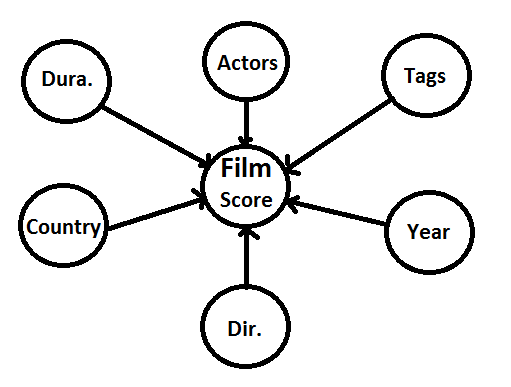
\includegraphics[width=0.5\linewidth]{images/Modelo}
		 	\caption{Modelo de película.}
		 	\label{fig:ModeloPelicula}
		\end{figure}
		El modelo va adaptándose cuando aparecen los usuarios, generando una nueva entidad por usuario y relacionado siempre por las películas en las cuáles tengan un mayor calificación, dependiendo de sus otros parámetros como año, director, etc.
		El modelo queda de la siguiente manera. Dentro del nodo usuario tendríamos la información de la cuenta como el correo electrónico o el hash de la contraseña.
		
		\begin{figure}[tbph!]
			\centering
			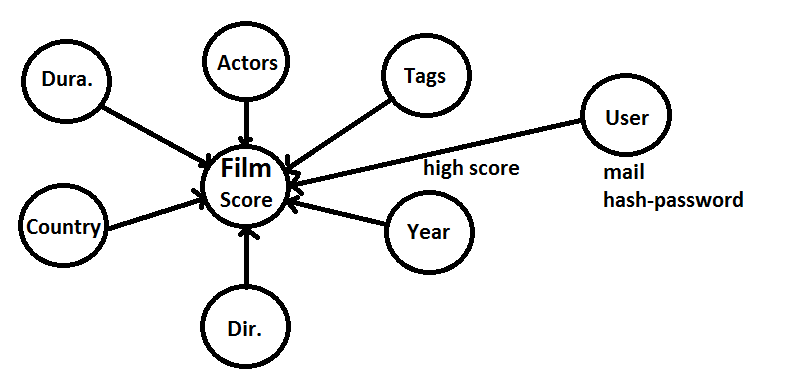
\includegraphics[width=0.5\linewidth]{images/Modelo_con_usuario}
			\caption{Modelo de película.}
			\label{fig:ModeloPelicula}
		\end{figure}
		
		\clearpage
		\section{Explicación del Frontend implementado}
		Por falta de medios no se ha podido implementar toda la solución completa, por lo que en este apartado voy a explicar como sería la aplicación en cuestión y como la hubiera desarrollado.\\
		
		Toda la aplicación estaría echa en AngularJS y para la parte de visualización del grafo se implementaría con D3.js. La página de Login sería la siguiente:
		
		\begin{figure}[tbph!]
			\centering
			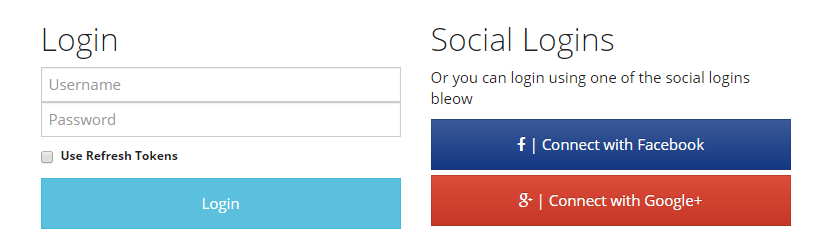
\includegraphics[width=0.7\linewidth]{images/Login}
			\caption{Página de Login.}
			\label{fig:Login}
		\end{figure}
		
		Una vez el usuario entre en la aplicación, tendremos una página inicio con las primeras recomendaciones para ese usuario basadas por la calificación. El usuario será el que diga si le gustan o no esas películas para que a través de las acciones que realice el usuario generemos nuevas recomendaciones.
		Dentro de cada película podremos ver toda su información. 
		\begin{figure}[tbph!]
			\centering
			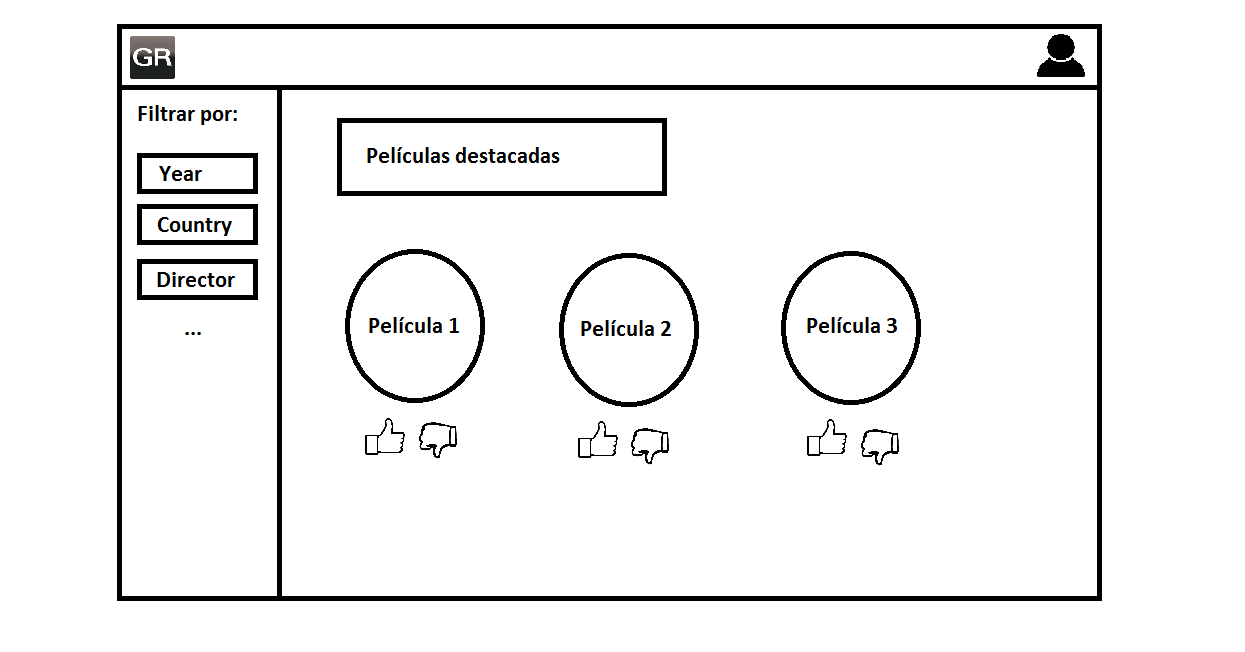
\includegraphics[width=0.7\linewidth]{images/Pagina_Inicio}
			\caption{Página de Inicio.}
			\label{fig:Inicio}
		\end{figure}
		
		
		\clearpage
		\section{Explicación del Backend implementado}
		El backend implementado es la base de datos Neo4j, la versión Community. Nos comunicaremos con ella a través de API realizando peticiones en Cypher.\\
		
		Como hemos visto anteriormente generaremos la base de datos de manera estática con las películas de Filmaffinity según el modelo propuesto.\\
		
		Cuando se genera un nuevo usuario, se realiza a siguiente consulta en Cypher.
		\begin{verbatim}
		CREATE (:USER {user:"NombreUsuario",
		hash:"HashContraseña", correo:"CorreoElectronico"})
		\end{verbatim}
		
		Después, para generar las primeras recomendaciones basadas en la calificación, realizaremos la siguiente consulta
		
		\begin{verbatim}
		MATCH (f:FILM) RETURN f.name as NOMBRE,
		f.score as CALIFICACION 
		order by  f.score desc limit 10
		\end{verbatim}
		
		Esto devolverá las 10 mejores películas según Filmaffinity. Tendremos que procesar la salida para poder mostrársela al usuario pero por falta de tiempo.\\
		
		\begin{figure}[tbph!]
		\centering
		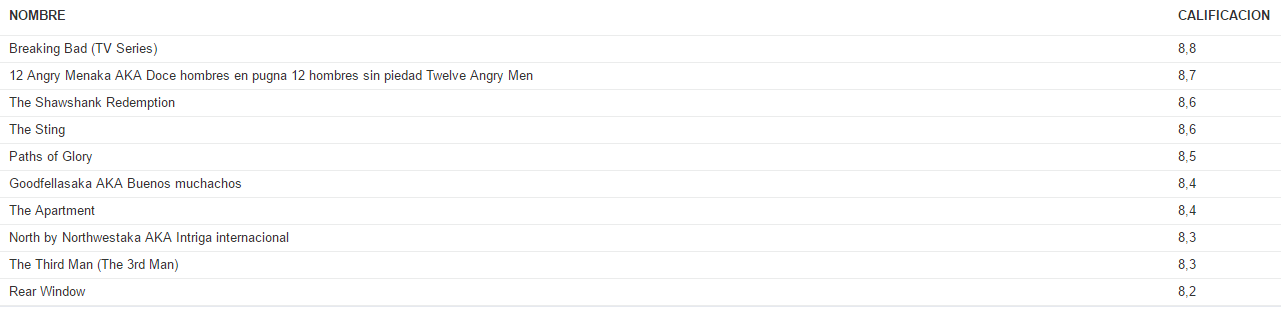
\includegraphics[width=0.9\linewidth]{images/BestFilms}
		\caption{Mejores Películas.}
		\label{fig:MejoresPeliculas}
		\end{figure}
		
		Si el usuario realiza la acción de "Me gusta" sobre una película, se creará una relación con ella de la siguiente manera.
		
		\begin{verbatim}
		MATCH (u:USER {user:"NombreUsuario"}), 
		(f:FILM {name:"NombrePelicula"}) 
		MERGE (u)-[:MEGUSTA {time:"timestamp"}]->(f)
		\end{verbatim}
		
		Si le diera a ``No me gusta'' se realizaría la acción de generar un nuevo parámetro de no mostrar con ella y se dejaría de mostrar.
		Si se le diera a ``No me gusta'' a una película que con anterioridad se le dio a me gusta se eliminaría esa relación.\\
		
		\begin{verbatim}
		MATCH (u:USER {user:"NombreUsuario"})-[r:MEGUSTA]-> 
		(f:FILM {name:"NombrePelicula"}) 
		DELETE r
		\end{verbatim}
		
		Cada vez que se realice la acción de ``Me gusta'' se realizan las diferentes consultas para seguir mostrando nuevas que estén relacionadas con sus parámetros. Un ejemplo de la consulta sería.\\
		
		\begin{verbatim}
		MATCH (f:FILM {name:"NombrePelicula"})
		with f
		MATCH (f)<--(:YEAR)-->(f1:FILM) 
		RETURN f1
		\end{verbatim}
		\clearpage
		\section{Demostración mediante ejemplos}
		Ejemplo tonto de demo
		Base de datos neo4j con varios usuarios.
	
\end{document}
